\documentclass[12pt]{article}
% \usepackage[T1]{fontenc}
% \usepackage{calc}
% \usepackage{hyperref}\usepackage{setspace}
% \usepackage{multicol}
% \usepackage[normalem]{ulem}
\usepackage{color}
\usepackage{alltt}
\usepackage{graphicx}           %For graphics

\usepackage{listings}           %Guido's code listings package

\lstloadlanguages{Java}
\lstset{language=Java,
%  frameround=tttt,
%  frame=trBL,
%  basicstyle={\ttfamily,\footnotesize},
  basicstyle=\ttfamily\scriptsize,
%  basicstyle=\footnotesize,
  commentstyle=\itshape,
  lineskip=-2pt,
%  stringspaces=f,
  escapechar=@
}
 
% \setlength{\oddsidemargin}{1.0000in-1in}
% \setlength{\textwidth}{\paperwidth - 1.0000in-1.0000in}


\begin{document}
\section{GAIGS ``as is'' -- that is, without extending its built-in data structure visuals}

The GAIGS (Generalized Algorithm Illustration via Graphical Software)
is an algorithm visualization scripting language that captures and
renders snapshots of the state of an algorithm at interesting
events--critical points in its execution.

%\subsection{The textual algorithm visualizations read by GAIGS}


The series of snapshots to be rendered by GAIGS is represented in XML.
While GAIGS uses the file extension .sho for storing and reading its
visualizations, the files are simply .xml files under a different
name. When GAIGS loads one of these .sho files, the XML contained
within is validated against its DOCTYPE, if one is provided. The
built-in structures are all checked against the file gaigs\_sho.dtd,
and these are the structures that will be covered first.

(This introduction to GAIGS will assume the reader has a basic
understanding of XML and DTD's.)

% Introductions to XML and DTD's can be
% found in many places, for example online at W3 Schools
% (http://www.w3schools.com).)



\subsection{The ``data type definition'' for GAIGS script, as specified in gaigs\_sho.dtd}


The root element of a .sho file is the ``show''.

\footnotesize \begin{verbatim}
  <!ELEMENT show (snap+, questions?)>
\end{verbatim} \normalsize
  
A show consists of one or more snaps, optionally followed by
questions. Questions will be covered later, but they are an
important way of ensuring that someone viewing an algorithm
visualization will be actively participating.


Here is the definition of a ``snap'':

\footnotesize \begin{verbatim}
  <!ELEMENT snap (title, doc_url?, pseudocode_url?,
                  (tree|array|graph|stack|queue|linkedlist|bargraph)*,question_ref?)>
\end{verbatim} \normalsize

\begin{description}
\item[title:]  The title element is simply \#PCDATA. It can consist of
  multiple lines of text, and these lines of text appear centered at
  the top of a snapshot.
  

\item [doc\_url:] The URL of the text that can be viewed in the Info
  tab as the visualization is running. 

  
\item [pseudocode\_url:] This is the same as the doc\_url element,
  except the text can be viewed under the pseudocode tab when running
  a visualization.  (If the Webserver you are using supports PHP,
  extensive support is provided to dynamically highlight lines of code
  -- see Section \ref{pseudocode-win})
  
  
\item [structures:] After the title and the two optional URLs comes
  zero or more structures. (These are all implemented in Java and
  descend from the abstract class StructureType -- see Section
  \ref{extending-gaigs}.) Each of these structure types is defined in
  the DTD. They will be discussed next.
  

\item [question\_ref]: Finally comes the question\_ref. The question\_ref
  element is empty, and has one CDATA attribute: ``ref''. This
  corresponds to a question element's ``id'' (covered later).

\end{description}

% The basic framework of a  visualization .sho file


Here is an example of the most basic visualization GAIGS can produce:

\footnotesize \begin{verbatim}
<?xml version="1.0" encoding="UTF-8"?>
<!DOCTYPE show PUBLIC "-//JHAVE//DTD GAIGS SHO//EN" "gaigs_sho.dtd">

<show>
  <snap>
    <title>Hello World</title>
  </snap>
</show>
\end{verbatim} \normalsize

This will produce a show with a single snapshot, containing nothing more than the title, ``Hello World'':

\begin{center}
  
\includegraphics[width=3in]{howto_graphics/helloworld.eps}
\end{center}


\subsubsection{A structure's ``name'' element}


All built-in structures have an optional ``name'' element. It contains
nothing more than \#PCTEXT. When drawing multiple structures to
different areas of the screen, the structure's ``name'' element
provides a simple and basic way of labeling the structure. However, if
the structure is drawn in or near default bounds (the unit square),
the structure's name may collide with the title for the entire
snapshot as they are both drawn in the same way.



\subsubsection{A structure's ``bounds'' element}


All built-in structures also have the optional ``bounds'' element. Here is its definition:

\footnotesize \begin{verbatim}
<!ELEMENT bounds (EMPTY)>
<!ATTLIST bounds x1 CDATA #REQUIRED
                 y1 CDATA #REQUIRED
                 x2 CDATA #REQUIRED
                 y2 CDATA #REQUIRED
                 fontsize CDATA "0.03">
\end{verbatim} \normalsize


                 
The ``x1'' and ``y1'' attributes are the coordinates
of the lower-left corner, and the ``x2'' and ``y2''
correspond to the upper-right corner. The
``fontsize'' attribute can be adjusted to make text
readable when a structure is drawn to a smaller
portion of the screen. The default value is 0.03
(which is, in a rough sense, 3\% of the height of the
screen).



\subsubsection{Colors in GAIGS}


The built-in structures allow nodes, cells, and connecting lines to be
colored independently from each other. The colors can be selected from
a predefined set of colors, or through hexadecimal notation.  The
predefined colors are: white, black, red, green, blue, yellow,
magenta, light blue

The hex format is a '\#' character followed by six hex digits. The hex
digits describe the color in standard RGB fashion: \#RRGGBB.


\footnotesize \begin{verbatim}
  #000000  <- black
  #FF0000  <- bright red
  #00AA00  <- green
  #000055  <- dark blue
  #888888  <- grey
  #FFFFFF  <- white
\end{verbatim} \normalsize


\subsubsection{The stack, queue, and linkedlist structure types}


The stack, queue, and linkedlist structure types all have the same syntax:

\footnotesize \begin{verbatim}
  <!ELEMENT stack      (name?, bounds?, list_item*)>
  <!ELEMENT queue      (name?, bounds?, list_item*)>
  <!ELEMENT linkedlist (name?, bounds?, list_item*)>
\end{verbatim} \normalsize
  
  The name and bounds are common to all structures.  The stack, queue,
  and linkedlist structures all have zero or more list\_items, each of
  which represents an entry in the data structure. A list\_item is
  simply:

\footnotesize \begin{verbatim}
  <!ELEMENT list_item (label)>
  <!ATTLIST list_item color CDATA "#FFFFFF">
\end{verbatim} \normalsize
  
  This describes a ``label'' for the cell (element containing only
  \#PCDATA), and a CDATA attribute ``color'' describing the background
  color of the cell.  The color of the label text is automatically
  determined to make the text readable.

The list\_item given first will serve as the top of a stack, the head
of a linkedlist, or the front of a queue. The subsequent list\_items
then come in order with the last one serving as the bottom, tail, or
back of the data structure.

Here is an example stack. Changing the structure's tag (and the
closing tag) name from ``stack'' to ``queue'' or ``linkedlist'' will
be sufficient to produce a different data structure.

\footnotesize \begin{verbatim}
<?xml version="1.0" encoding="UTF-8"?>
<!DOCTYPE show PUBLIC "-//JHAVE//DTD GAIGS SHO//EN" "gaigs_sho.dtd">

<show>
  <snap>
    <title>An example stack</title>
    <stack>
      <list_item color="#000000">
        <label>Item A</label>
      </list_item>
      <list_item color="#888888">
        <label>Item B</label>
      </list_item>
      <list_item color="#888888">
        <label>Item C</label>
      </list_item>
    </stack>
  </snap>
</show> 
\end{verbatim} \normalsize

Given this code, GAIGS produces a show consisting of a single
snapshot, titled ``An example stack''. A three-element stack is
centered on the drawing area with Item A on top, B in the middle, and
Item C on the bottom. This stack has colored items, with Item A's
background color as black and the other two's color as a shade of
grey.


\begin{center}
  
\includegraphics[width=3in]{howto_graphics/stack.eps}
\end{center}


\subsubsection{The array structure type}


The array structure type is defined as follows:

\footnotesize \begin{verbatim}
  <!ELEMENT array (name?, bounds?, row_label*, column_label*, column*)>

  <!ELEMENT row_label (#PCDATA)> <!-- put in empty titles if you want to skip titling some rows -->
  <!ELEMENT column_label (#PCDATA)>

  <!ELEMENT column (list_item*)>
\end{verbatim} \normalsize
  
  As with all other built-in structures, the first two elements are
  the optional name and bounds.  The next set of entries is zero or
  more row\_labels (which are element containing only \#PCDATA). These
  are drawn to the left of the array, with the first one appearing at
  the top, or row index 0. The column\_labels are handled similarly,
  with the first appearing at the left, or column index 0. The final
  entry in an array is a set of zero or more columns. Each column
  consists of zero or more list\_items, which are the same as the
  list\_items used in stacks, queues, and linkedlists.

Here is an example 3x2 array.

\footnotesize \begin{verbatim}
<?xml version="1.0" encoding="UTF-8"?>
<!DOCTYPE show PUBLIC "-//JHAVE//DTD GAIGS SHO//EN" "gaigs_sho.dtd">

<show>
  <snap>
    <title>An example 3x2 array</title>
    <array>
      <row_label>Row 0</row_label>
      <row_label>Row 1</row_label>
      <row_label>Row 2</row_label>
      <column_label>Col0</column_label>
      <column_label>Col2</column_label>
      <column>
        <list_item>
          <label>[0][0]</label>
        </list_item>
        <list_item>
          <label>[1][0]</label>
        </list_item>
        <list_item color="red">
          <label>[2][0]</label>
        </list_item>
      </column>
      <column>
        <list_item>
          <label>[0][1]</label>
        </list_item>
        <list_item>
          <label>[1][1]</label>
        </list_item>
        <list_item>
          <label>[2][1]</label>
        </list_item>
      </column>
    </array>
  </snap>
</show>
\end{verbatim} \normalsize

And here is the one-snapshot show that GAIGS will produce from this code:


\begin{center}
  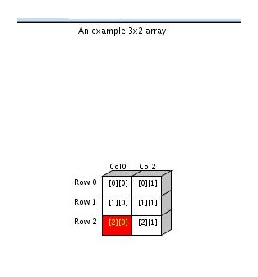
\includegraphics[width=3in]{howto_graphics/array.eps}
\end{center}


\subsubsection{The bargraph structure type}


The bargraph is a simple structure:

\footnotesize \begin{verbatim}
  <!ELEMENT bargraph (name?, bounds?, bar*)>

  <!ELEMENT bar (EMPTY)>
  <!ATTLIST bar magnitude CDATA #REQUIRED
                color CDATA "#000000">
\end{verbatim} \normalsize
  
  After the standard name and bounds elements comes zero or more
  ``bar'' elements. These bar elements are empty, but possess two
  attributes: a magnitude and a color. The range of (positive) values
  used for magnitudes does not matter as the structure will scale the
  height of the bars drawn to the screen accordingly -- with the bar
  of greatest magnitude extending for the entire vertical bounds of
  the structure. The first bar given will be the one furthest on the
  left. Here is code for an example bargraph, followed by the image
  GAIGS produces when fed the code. This example uses the optional
  ``bounds'' element to resize the bargraph to insure that the largest
  bar does not extend for the entire vertical length of the snapshot's
  drawing window. The workings of the bounds element will be
  explained later.

\footnotesize \begin{verbatim}
<?xml version="1.0" encoding="UTF-8"?>
<!DOCTYPE show PUBLIC "-//JHAVE//DTD GAIGS SHO//EN" "gaigs_sho.dtd">

<show>
  <snap>
    <title>An example bargraph</title>
    <bargraph>
      <bounds x1="0.2" y1="0.1" x2="0.8" y2="0.75"/>
      <bar magnitude="64"  color="red"/>
      <bar magnitude="255" color="green"/>
      <bar magnitude="128" color="blue"/>
    </bargraph>
  </snap>
</show>
\end{verbatim} \normalsize


\begin{center}
  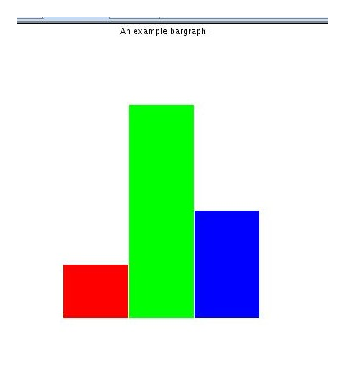
\includegraphics[width=3in]{howto_graphics/bargraph.eps}
\end{center}


\subsubsection{The tree structure type}


The tree structure comes in two varieties: general and binary. While a
binary tree may be a special case of a general tree, at times it is
be necessary to indicate visually whether a solitary child is the left
or right child of its parent. Here is the base of the tree structure:


\footnotesize \begin{verbatim}
  <!ELEMENT tree (name?, bounds?, (tree_node|binary_node)? )>
  <!ATTLIST tree x_spacing CDATA "1.5"
                 y_spacing CDATA "1.5">
\end{verbatim} \normalsize
  
  After the standard name and bounds elements comes either a
  tree\_node, which serves as the root of a general tree, or a
  binary\_node, which serves as the root of a binary tree. The
  ``tree'' element also has two attributes, x\_ and y\_spacing. These
  control how far apart the nodes of the tree are spread in the x-
  and y-directions. The number is interpreted as a multiple of the
  diameter of the nodes (the nodes are sized to fit the text inside).
  The distance is measured from the center of each node, so the
  default values of 1.5 will result in the outer edges of the nodes
  being separated vertically and horizontally by one half of the
  nodes' diameters.

Here is the definition of a general tree's tree\_node:


\footnotesize \begin{verbatim}
  <!ELEMENT tree_node (label?, (tree_node,tree_edge?)* )>
  <!ATTLIST tree_node color CDATA "white">
\end{verbatim} \normalsize

As you can see, each tree\_node has a label (a \#PCDATA element), and
can have zero or more children tree\_nodes, each followed by an
optional tree\_edge element describing how the parent is connected to
the child coming immediately before the tree\_edge. The tree\_nodes also
have a ``color'' attribute. The nodes are drawn on the tree from left
to right.

The binary\_node looks like this:

\footnotesize \begin{verbatim}
  <!ELEMENT binary_node (label?, (left_node,tree_edge?)?, (right_node,tree_edge?)? )>
  <!ATTLIST binary_node color CDATA "white">
\end{verbatim} \normalsize  

The binary\_node has a label, followed by zero, one, or two children
nodes. The definitions for left\_node and right\_node are identical to
the definition for the binary node. The difference in names only
serves to identify a node as the left or right child of its parent.
The optional tree\_edges behave the same way in the binary tree as in
the general tree: they describe the edge connecting the parent to the
child that comes immediately before the description.

Here is the definition of the tree\_edge element, used by both the
tree\_nodes and binary\_nodes:

\footnotesize \begin{verbatim}
  <!ELEMENT tree_edge (label?)>
  <!ATTLIST tree_edge color CDATA "black">
\end{verbatim} \normalsize

The edges can be labeled (\#PCDATA element) and/or colored.

Here is code for an example general tree, with one of the nodes
highlighted light blue. The picture shows how GAIGS renders this.

\footnotesize \begin{verbatim}
<?xml version="1.0" encoding="UTF-8"?>
<!DOCTYPE show PUBLIC "-//JHAVE//DTD GAIGS SHO//EN" "gaigs_sho.dtd">

<show>
  <snap>
    <title>An example tree</title>
    <tree>
      <tree_node color="light blue">     <!--  The root node labeled A-->
        <label>A</label>
        <tree_node>                      <!--  B1 is a child of A -->
          <label>B1</label>
          <tree_node>                    <!--  C is a child of B1 -->
            <label>C</label>
          </tree_node>
        </tree_node>
        <tree_node>                      <!--  B2 is a second child of A -->
          <label>B2</label>
        </tree_node>
      </tree_node>
    </tree>
  </snap>
</show>
\end{verbatim} \normalsize


\begin{center}
  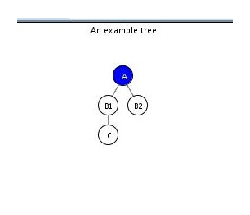
\includegraphics[width=3in]{howto_graphics/generaltree.eps}
\end{center}


Here is code for an example binary tree, with labeled edges and a
colored edge. This code is also followed by an image.

\footnotesize \begin{verbatim}
<?xml version="1.0" encoding="UTF-8"?>
<!DOCTYPE show PUBLIC "-//JHAVE//DTD GAIGS SHO//EN" "gaigs_sho.dtd">

<show>
  <snap>
    <title>An example binary tree</title>
    <tree x_spacing="2.0" y_spacing="2.0">
      <binary_node>                  <!--  A hyphen in the root -->
        <label>-</label>  
        <left_node>                  <!--  0 the left child of the root -->
          <label>0</label>  
          <right_node>               <!--  01 the right child of 0 -->
            <label>01</label>
          </right_node>
          <tree_edge color="red">
            <label>1</label>
          </tree_edge>
        </left_node> 
        <tree_edge>
          <label>0</label>
        </tree_edge>
        <right_node>                 <!--  1 is right child of the root -->
          <label>1</label>
        </right_node>
        <tree_edge>
          <label>1</label>
        </tree_edge>
      </binary_node>
    </tree>
  </snap>
</show>
\end{verbatim} \normalsize

\begin{center}
  
\includegraphics[width=3in]{howto_graphics/binarytree.eps}
\end{center}


\subsubsection{The graph structure type}

The graph structure type can also be used to draw a network (that is,
a graph with weighted edges). Here is the first part of the definition
of a graph:

\footnotesize \begin{verbatim}
  <!ELEMENT graph (name?, bounds?, vertex*)>
  <!ATTLIST graph weighted (true|false) "false">
\end{verbatim} \normalsize

After the standard name and bounds elements, a graph has a set of zero
or more vertex elements. A graph also has an attribute ``weighted''.
If ``weighted'' is set to ``true'', the graph will load and draw edge
weights.

Here is the definition of the vertex elements:

\footnotesize \begin{verbatim}
  <!ELEMENT vertex (label?, position?, edge*)>
  <!ATTLIST vertex color CDATA "white"
                   id CDATA #REQUIRED>
\end{verbatim} \normalsize
  
  Each vertex can have a label (\#PCDATA element). Then comes an
  optional position element, telling GAIGS where to draw the node. If
  the positions of the vertices are not specified, GAIGS arranges the
  vertices equally spaced around the circumference of a circle. This
  works well for small numbers of vertices, but for larger numbers it
  may be best to specify the vertices' positions using a graph vertex
  placement algorithm. GAIGS uses normalized screen coordinates to
  describe positions, so the coordinates should be between 0 and 1.
  Here is what the position element looks like:

\footnotesize \begin{verbatim}
  <!ELEMENT position (EMPTY)>
  <!ATTLIST position x CDATA #REQUIRED
                     y CDATA #REQUIRED>
\end{verbatim} \normalsize

After the position element comes a set of zero or more edges. Each
vertex has an ``id'' attribute that must be different from all other
vertices' id's in the graph. The edge's ``target'' attribute should
match the id of the vertex it connects to. Here is the definition of a
vertex's edge:

\footnotesize \begin{verbatim}
  <!ELEMENT edge (label?)>
  <!-- target is matched with vertex.id: -->
  <!ATTLIST edge target CDATA #REQUIRED
                 directed (true|false) "false"
                 color CDATA "#999999"> <!-- grey -->
\end{verbatim} \normalsize

If the ``directed'' attribute is set to true, an arrow is drawn on the
edge pointing from the current vertex to the target. The edge can be
labeled, if the graph's ``weighted'' attribute is set to true.
Finally, the edge's color can be defined.

Here is the code for an example weighted graph (network), followed by
an image of how GAIGS renders the code. (Note: As of August, 2005, the
self-connecting edges are not being rendered properly, but 
luck this bug/feature should soon be resolved.)

\footnotesize \begin{verbatim}
<?xml version="1.0" encoding="UTF-8"?>
<!DOCTYPE show PUBLIC "-//JHAVE//DTD GAIGS SHO//EN" "gaigs_sho.dtd">

<show>
  <snap>
    <title>An example weighted graph (network)</title>
    <graph weighted="true">
      <vertex color="#FF8855" id="A">
        <label>A</label>
        <position x="0.2" y="0.2"/>
        <edge target="B" color="#00FF00">  <!--  Bi-directional edge between A and B -->
          <label>5</label>
        </edge>
        <edge target="C" directed="true">  <!--  Directional edge from A to C -->
          <label>8</label>
        </edge>
      </vertex>
      <vertex color="#FF2222" id="B">
        <label>B</label>
        <position x="0.7" y="0.7"/>
        <edge target="B" color="red">     <!--  See Note above regarding self-connecting edges -->
          <label>1</label>
        </edge>
        <edge target="D">                 <!--  Bi-directional edge between B and D -->
          <label>3</label>
        </edge>
      </vertex>
      <vertex color="#DD9922" id="C">
        <label>C</label>
        <position x="0.2" y="0.7"/>
      </vertex>
      <vertex color="#AA77AA" id="D">
        <label>D</label>
        <position x="0.7" y="0.2"/>
      </vertex>
    </graph>
  </snap>
</show>
\end{verbatim} \normalsize



\begin{center}
  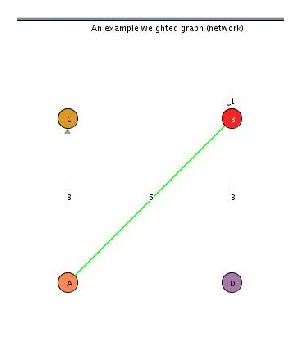
\includegraphics[width=3in]{howto_graphics/graph.eps}
\end{center}


\subsubsection{The bounds element and drawing more than one structure to a snapshot}


All the built-in structures have an optional bounds element that can
be used to position and resize structures. Here is the definition of
the bounds element:

\footnotesize \begin{verbatim}
  <!ELEMENT bounds (EMPTY)>
  <!ATTLIST bounds x1 CDATA #REQUIRED
                   y1 CDATA #REQUIRED
                   x2 CDATA #REQUIRED
                   y2 CDATA #REQUIRED
                   fontsize CDATA "0.03">
\end{verbatim} \normalsize
  
  The first four attributes define the coordinates of a rectangle that
  the structure will consider the bounds of where it is allowed to
  draw itself. The x1,y1 pair corresponds to the lower-left corner,
  and the x2,y2 pair corresponds to the upper-right corner. (It should
  be noted that not all features are rendered distortion-free when the
  height-to-width ratio is not one-to-one. For example, having a
  scaled height of 1.0 but a scaled width of 0.5 may create distortion
  in a vertical direction.) After the four coordinate attributes comes
  an optional fontsize attribute. Scaling a structure into a quarter
  of the area of the screen may make text so small as to be unreadable, but
  increasing the fontsize will solve that problem. The fontsize
  defaults to 0.03, which is in a rough sense 3\% of the height of the
  GAIGS window at the default zoom level.

Here is the code for an example snapshot that resizes and positions
two structures on the screen simultaneously:

\footnotesize \begin{verbatim}
<?xml version="1.0" encoding="UTF-8"?>
<!DOCTYPE show PUBLIC "-//JHAVE//DTD GAIGS SHO//EN" "gaigs_sho.dtd">

<show>
  <snap>
    <title>The heap datastructure</title>
    <tree>                              <!--  First a tree view -->
      <name>The heap visually</name>
      <bounds x1="0.0" y1="0.2" x2="0.5" y2="0.7" fontsize="0.06"/>
      <binary_node>
        <label>A</label>
        <left_node>
          <label>B</label>
          <left_node>
            <label>D</label>
          </left_node>
        </left_node>
        <right_node>
          <label>C</label>
        </right_node>
      </binary_node>
    </tree>
    <array>                            <!--  Then the underlying array for the heap -->
      <name>The heap in memory</name>
      <bounds x1="0.5" y1="0.2" x2="1.0" y2="0.7" fontsize="0.06"/>
      <column>
        <list_item>
          <label>A</label>
        </list_item>
        <list_item>
          <label>B</label>
        </list_item>
        <list_item>
          <label>C</label>
        </list_item>
        <list_item>
          <label>D</label>
        </list_item>
      </column>
    </array>
  </snap>
</show>
\end{verbatim} \normalsize


\begin{center}
  
\includegraphics[width=3in]{howto_graphics/bounds.eps}
\end{center}


% \subsubsection{(Pseudocode and Documentation URL's: sort of explained already)}



\subsubsection{Snapshot questions in GAIGS}


Each snapshot can have a question\_ref element. A question\_ref
element comes at the end of the snapshot. It is empty and has an
attribute ``ref'' whose value should match the ``id'' attribute of
some question. The individual question elements (and their correct
answers) come at the end of the ``show'' element, collected inside a
``questions'' element. The ``questions'' element is simply zero or
more question elements:


\footnotesize \begin{verbatim}
  <!ELEMENT questions (question*)>
\end{verbatim} \normalsize

Each question has two required attributes, the text of the question, and zero or more answer options:

\footnotesize \begin{verbatim}
  <!ELEMENT question (question_text,answer_option*)>
  <!ATTLIST question type CDATA #REQUIRED
                     id CDATA #REQUIRED>
    <!-- type: MCQUESTION|TFQUESTION|FIBQUESTION|MSQUESTION -->
\end{verbatim} \normalsize
  
  The question's id should be unique from all other question id's and
  should match a snap's question\_ref's ``ref'' attribute. The
  question's type must be one of the four question types provided,
  which are listed above in the comment: multiple-choice,
  true-or-false, fill-in-the-blank, or multiple-selection (check all
  of the possible answers which are correct). The question\_text is
  simply \#PCDATA:

\footnotesize \begin{verbatim}
  <!ELEMENT question_text (#PCDATA)> <!-- the quesiton to ask the user -->
\end{verbatim} \normalsize

Here is the definition for the answer\_option elements:

\footnotesize \begin{verbatim}
  <!ELEMENT answer_option (#PCDATA)>
     <!-- TFQuestion: use text "true" or "false" (no quotes) for the correct answer -->
  <!ATTLIST answer_option is_correct (yes|no) "no">
    <!-- specify "yes" only if it is a MC/MSQuestion. otherwise, ignored -->
\end{verbatim} \normalsize

For multiple-choice and multiple-selection questions, the
answer\_options listed in the question will be the possible choices to
choose from when the question is asked. To define which is the correct
answer, set the ``is\_correct'' attribute of the answer\_option to yes
or no (a multiple-choice question should only have one correct
answer). For fill-in-the-blank questions, simply provide in the
answer\_options' text acceptable answers (case-insensitive). For
true-or-false questions, provide only one answer\_option element with
the text set to either ``true'' or ``false'' (no quotes). The
MSQUESTION and MCQUESTION are the only types that care about the
answer\_options' ``is\_correct'' attribute; both the FIBQUESTION and
TFQUESTION ignore this attribute.

Here is the code for an example GAIGS show that asks a question of
each of the four types. Each of the four snapshots contains nothing
but a question\_ref (and the required title). The structures would be
added between the title and question\_ref elements.

\footnotesize \begin{verbatim}
<?xml version = "1.0" encoding = "UTF-8"?>
<!DOCTYPE show PUBLIC "-//JHAVE//DTD GAIGS SHO//EN" "gaigs_sho.dtd">

<show>

 <snap>
  <title>Question 1</title>
  <question_ref ref="k"/>
 </snap>

 <snap>
  <title>Question 2</title>
  <question_ref ref="222"/>
 </snap>

 <snap>
  <title>Question 3</title>
  <question_ref ref="abc"/>
 </snap>

 <snap>
  <title>Question 4</title>
  <question_ref ref="msq"/>
 </snap>

 <questions>
  <question type="TFQUESTION" id="k">
   <question_text>This statement is a question.</question_text>
   <answer_option>false</answer_option>
  </question>
  <question type="FIBQUESTION" id="222">
   <question_text>The answer to the ultimate question of life, the universe, and everything is:</question_text>
   <answer_option>42</answer_option>
   <answer_option>forty-two</answer_option>
   <answer_option>pie</answer_option>
  </question>
  <question type="MCQUESTION" id="abc">
   <question_text>"McQuestion" sounds like an item on the menu of:</question_text>
   <answer_option is_correct="yes">McDonald's</answer_option>
   <answer_option is_correct="no">Hardee's</answer_option>
   <answer_option>Burger King</answer_option>
   <answer_option>Pizza Hut</answer_option>
  </question>
  <question type="MSQUESTION" id="msq">
   <question_text>"Which numbers are prime?"</question_text>
   <answer_option is_correct="no" >0</answer_option>
   <answer_option is_correct="no" >1</answer_option>
   <answer_option is_correct="yes">2</answer_option>
   <answer_option is_correct="yes">3</answer_option>
   <answer_option is_correct="no" >4</answer_option>
   <answer_option is_correct="yes">5</answer_option>
  </question>
 </questions>

</show>
\end{verbatim} \normalsize


The first question is true-or-false. The text of the question reads,
``This statement is a question.'' The correct answer is specified
between a set of answer\_option tags: false. 

The second question is fill-in-the-blank. The text of the question
reads, ``The answer to the ultimate question of life, the universe,
and everything is:'' The answers accepted as correct are ``42'',
``forty-two'', and ``pie''.

The third question is multiple-choice. The text of the question reads,
``McQuestion" sounds like an item on the menu of:'' Four answer
options are provided, with the first being correct.

The fourth question is multiple-selection. The text of the question
reads, ``Which numbers are prime?'' Six answer options are provided,
with the third, fourth, and sixth being correct.


\section{Creating your own structure types in GAIGS}
\label{extending-gaigs}

If you don't like GAIGS's built-ins, you do what every OO programmer
does -- extend and plug-in!

The first step is to decide on the XML for your extension.  That will
essentially define its syntax in a show.  To illustrate, below we add
a \textit{foobar} element to the possible elements appearing in a
\verb'<'snap\verb'>' tag:

\footnotesize \begin{verbatim}
<!ELEMENT show (snap+, questions?)>

<!ELEMENT snap (title, doc_url?, pseudocode_url?, 
         (tree|array|graph|stack|queue|linkedlist|bargraph|foobar)*,question_ref?)>

<!ELEMENT title (#PCDATA)>
<!ELEMENT name  (#PCDATA)>
<!ELEMENT label (#PCDATA)>
<!ELEMENT doc_url (#PCDATA)>
<!ELEMENT pseudocode_url (#PCDATA)>

<!ELEMENT bounds (EMPTY)>
<!ATTLIST bounds x1 CDATA #REQUIRED
                 y1 CDATA #REQUIRED
                 x2 CDATA #REQUIRED
                 y2 CDATA #REQUIRED
                 fontsize CDATA "0.03">

     <!-- FOOBAR -->

<!ELEMENT foobar (name?, bounds?, nodelabel)>
<!ATTLIST foobar x CDATA "0.5"
               y CDATA "0.5"
               color CDATA "white">
<!ELEMENT nodelabel (EMPTY)>
<!ATTLIST nodelabel text CDATA "">
\end{verbatim} \normalsize

The rest of the DTD remains unchanged.
For example, consider a \verb'<'show\verb'>' adhering to this DTD and defining a ``foobar''.

\footnotesize \begin{verbatim}  
<?xml version="1.0" encoding="UTF-8"?>

<!-- <!DOCTYPE show PUBLIC "-//JHAVE//DTD GAIGS SHO//EN" "gaigs_sho.dtd"> --> 
<!-- Use local SYSTEM DTD instead of the PUBLIC DTD -->

<!DOCTYPE show SYSTEM "gaigs_sho.dtd">  

<show>
  <snap>
    <title>An example of a simple foobar</title>
    <foobar x="0.25" y="0.25" color="#FF0000">
      <name>foobar1</name>
      <bounds x1="0.2" y1="0.1" x2="0.8" y2="0.75"  fontsize="0.1"/>
      <nodelabel text="The first foobar"/>
    </foobar>
  </snap>

  <snap>
    <title>An example of two simple foobars</title>
    <foobar x="0.25" y="0.25" color="#0000FF">
      <name>foobar2</name>
      <bounds x1="0.0" y1="0.0" x2="0.45" y2="0.45"  fontsize="0.1"/>
      <nodelabel text="The second"/>
    </foobar>
    <foobar x="0.25" y="0.25" color="#00FF00">
      <name>foobar3</name>
      <bounds x1="0.45" y1="0.45" x2="0.9" y2="0.9" fontsize="0.1"/>
      <nodelabel text="The third"/>
    </foobar>
  </snap>

</show>
\end{verbatim}
\normalsize
  
In the source code for GAIGS, every data structure has
\textit{StructureType} as an ancestor.

\small
\begin{verbatim}
StructureType 
|-- Md_Array     
|-- LinearList   
    |-- Stack       
    |-- Queue       
    |-- LinkedList                  
    |-- Bar                         
|-- BinaryTree                   
|-- GeneralTree        
|-- Graph_Network     
    |-- Ggraph           
    |-- Network          
\end{verbatim}
\normalsize


Hence coding your own structure type in Java source code is as simple
as writing one file, the \textit{YourStructureName.java} file
containing the class \textit{YourStructureName}, which inherits at
some point from the abstract class \textit{StructureType}. Both of
these files will be located in the \textit{jhave2/gaigs/src/gaigs2/}
directory, which can be built by running ant from the
\textit{jhave2/gaigs/} directory.  The StructureType class is an
abstract base, as indicated in the following documentation:

\begin{lstlisting}{}
// All GAIGS Structures inherit from ...
abstract class StructureType {

    // StructureType has only one parameterless constructor.

    // All derived structures should provide their own parameterless
    // constructor and override the following two methods:
    
    // Load the structure from the root of its XML tree (JDOM style)
    void loadStructure(Element myRoot, LinkedList llist, draw d)  @\hfill \textcolor{black}{\fbox{Parse the script}}@

    // All derived StructureTypes should override this -- be sure to
    // call super on this method when your structure is empty
    void drawStructure (LinkedList llist, draw d)  @\hfill \textcolor{black}{\fbox{And render it \ldots}}@

    // *** USEFUL PROTECTED METHODS AND VARIABLES

    // Access your GKS graphics routines thru this. Send drawing commands
    // to this Localized GKS object in normalized [0,1]x[0,1] coordinates
    // describing your position within the bounds given to LGKS 
    protected LocalizedGKS LGKS;

    // For derived objects who want to know their bounds
    protected double structure_fontsize, structure_left, 
                     structure_right, structure_bottom, structure_top;


    // Load name and bounds info common to all localized derived structures
    public void load_name_and_bounds(Element my_root, LinkedList llist, draw d) 

    // Given s, return its normalized width  @\hfill \textcolor{black}{\fbox{Often used to size a box or circle around text}}@
    protected double normalized_width(String s) 

    // Given color as a (usually hex) string, convert it to the right
    // Java color as int
    protected int colorStringToInt(String color) 

    // Given a fill-area color as a (usually hex) string, convert text
    // to appear in the fill area to the right Java color as int
    protected int colorStringToTextColorInt(String color) 
\end{lstlisting}


\subsection{Your structure's LGKS object is what you ``draw'' with.}

\begin{lstlisting}{}
    // YOUR LGKS OBJECT RESPONDS TO THE FOLLOWING MESSAGES
    // The LinkedList and draw objects always tag along ...
   
    // Set the interior style for a fill area.  The int color is
    // typically obtained from the hex string by StructureType's
    // colorStringToInt method.  Sorry, only the constants bsClear and
    // bsSolid are presently supported for style.  And, of course, a
    // clear fill area is just ...
    public void set_fill_int_style(int style, int color, LinkedList seginfo, draw d) 

    // Draw a fill area with the specified number of points and their
    // coordinates
    public void fill_area(int numpts, double ptsx[], double ptsy[], 
                          LinkedList seginfo, draw d) 
    
    // Draw a polyline with the specified number of points and their
    // coordinates
    public void polyline(int numpts, double ptsx[], double ptsy[], 
                         LinkedList seginfo, draw d) 
    
    // Set the text alignment.  Choices for horiz and vert are:
    //     final static int TA_CENTER    = 0;   
    //     final static int TA_LEFT      = 1;
    //     final static int TA_RIGHT     = 2;
    // 
    //     final static int TA_BASELINE  = 0;
    //     final static int TA_BOTTOM    = 1;
    //     final static int TA_TOP       = 2;  
    public void set_text_align(int horiz, int vert, LinkedList seginfo, draw d) 

    // Set the color (as a Java int) for drawing text.  Usually this
    // int is obtained from the hex string by your having called
    // colorStringToTextColorInt in StructureType.java
    public void set_textline_color(int color, LinkedList seginfo, draw d) 

    // Change the font size
    public void set_text_height(double height, LinkedList seginfo, draw d) 
    
    // Draw your text at the specified coordinate
    public void text(double x,double y, String str, LinkedList seginfo, draw d) 
   
    // Draw an ellipse from start angle thru end angle
    public void ellipse(double x, double y, double stangle, double endangle, 
                        double xradius, double yradius,
                        LinkedList seginfo, draw d) 
 
    // Draw a (outlined) circle
    public void circle(double x, double y, double radius, LinkedList seginfo, draw d) 
    
    // Draw a filled circle
    public void circle_fill(double x, double y, double radius, 
                            LinkedList seginfo, draw d) 
\end{lstlisting}

\subsection{Use the JDOM XML (www.jdom.org) parsing class to write loadStructure}

The JDOM essentials you will need \ldots

\begin{itemize}
\item The Element class provides the type of nodes in the XML tree, e.g., 
  \begin{lstlisting}{}
  public void loadStructure(Element rootEl, LinkedList thingsToRender, draw drawerObj)
  \end{lstlisting}
  
\item Given an Element, you can use \textit{getChild} to get the first
  child and \textit{getChildren} to return a \textit{List} of children


\item \textit{getText} returns the text (as a String) of a node in the tree
\item \textit{getAttributeValue(String which-attrib)} return the value of a particular attribute
\end{itemize}

Here's the resulting \textit{foobar.java} file

\begin{lstlisting}{}
// foobar.java
// A sample (and simple) extension of the GAIGS StructureType

package gaigs2;
import java.awt.image.*;
import java.util.*; 
import org.jdom.*;

public class foobar extends StructureType {

    double circle_center_x, circle_center_y; // center coords
    double circle_rad;          // radius

    int circle_color;           // node color

    int circle_labelcolor;      // text color
    String circle_label;        // only set up for a single line of text
    
    // Must provide a parameterless constructor for instantiation via reflection
    public foobar() {
        super();                // necessary

        circle_color = White;   // our hex notation is "#RRGGBB"
        circle_labelcolor = Black;
        circle_label = null;
        circle_center_x = 0.50;
        circle_center_y = 0.50;
        circle_rad = 0.25;
    } // foobar()       


    // This initialization method gets passed a jdom.Element whose
    // name is "foobar".  So gaigs_sho.dtd must be modified, adding a
    // "foobar" element to the list of structure types a snap can
    // contain.
    public void loadStructure(Element rootEl, LinkedList thingsToRender, draw drawerObj) {
        // This call loads the name and bounds if your xml
        // structure-element has a name and/or bounds like the
        // built-in structures.
        load_name_and_bounds(rootEl, thingsToRender, drawerObj);

        // JDOM, AT LEAST AS MUCH AS WE NEED IT, IS EASY TO USE
        List children = rootEl.getChildren(); // getChildren returns a list
        Iterator iter = children.iterator(); // which we will iterate through

        Element labelEl;

        // NOTE: This is only an unnecessary illustrative loop, since
        // we could get what we want directly
        while( iter.hasNext() ) {
            Element child = (Element) iter.next(); // walk through the list of children

            if( child.getName().equals("name") ) {
                // Just showing we could get it if we wanted,
                //  but already done for us in load_name_and_bounds(..)
                String junkName;
                junkName = child.getText(); // get the text of this node in the XML tree
            }
            else if( child.getName().equals("bounds") ) {
                //  Just showing we could get it if we wanted,
                //  but already done for us in load_name_and_bounds(..)
                double junkBound;
                junkBound = Format.atof( child.getAttributeValue("x1") ); // get an attribute
            }
            else if( child.getName().equals("nodelabel") )
                labelEl = child; 
        } // End illustrative loop

        // In this example, we could get the element we want directly --
        labelEl = rootEl.getChild("nodelabel");
        
        // The XML is validated against the DTD, so if there is a
        // #REQUIRED attribute or a default value we can safely assume
        // it is there
        circle_center_x = Format.atof( rootEl.getAttributeValue("x") );
        circle_center_y = Format.atof( rootEl.getAttributeValue("y") );

        circle_color = colorStringToInt( rootEl.getAttributeValue("color") );

        if( labelEl != null ) {
            circle_label = labelEl.getAttributeValue("text");
            circle_labelcolor = colorStringToTextColorInt( rootEl.getAttributeValue("color") );
            circle_rad = (normalized_width(circle_label) + structure_fontsize) / 2.0;
        }
    } // loadStructure


    // Use the LGKS object to draw the structure
    public void drawStructure(LinkedList thingsToRender, draw drawerObj) {
        // draw the circle(filled)
        LGKS.set_fill_int_style(bsSolid, circle_color, thingsToRender, drawerObj);
        LGKS.circle_fill(circle_center_x, circle_center_y, circle_rad, thingsToRender, drawerObj);

        // draw the circle outline
        LGKS.set_textline_color(Black, thingsToRender, drawerObj);
        LGKS.circle(circle_center_x, circle_center_y, circle_rad, thingsToRender, drawerObj);

        // draw the label
        LGKS.set_textline_color(circle_labelcolor, thingsToRender, drawerObj);
        LGKS.set_text_align(TA_CENTER, TA_BOTTOM, thingsToRender, drawerObj);
        LGKS.text(circle_center_x, circle_center_y, circle_label, thingsToRender, drawerObj);
    } // drawStructure

} // class foobar
\end{lstlisting}


% To see an example of what is required to extend StructureType take a
% look at \textit{foobar.java}, which is also located in the
% \textit{jhave2/gaigs/src/gaigs2/} directory and defines a new
% \textit{foobar} structure.
% 
% 
% 
% 
% There are many comments in the
% file, as well as a miniature JDOM demo that should demonstrate
% everything you need to know about using JDOM to walk around and access
% an XML tree (the XML has already been parsed for you). Only three
% methods need to be written: the constructor (which should call the
% no-argument constructor of StructureType), the method
% loadStructure(jdom.Element, LinkedList, draw), and the method
% drawStructure(LinkedList, draw). Your class need not worry about the
% LinkedList and draw arguments, other than to pass them on to other
% methods that do the actual work of drawing things.
% 
% A file called draw.java controls the matching of a structure's XML
% element name to the structure's Java class name. If no change is made
% to this file, the name of your structure in XML must exactly match
% (case-sensitive) the name of your structure in Java. If you wish to
% use a different name, you must modify the method assignStructureType
% that takes a jdom.Element as an argument. In that method you will find
% a comment showing exactly what to do, but the code is fairly
% straightforward: simply add a case for your structure name to the
% string of else-ifs.
% 
% At this point the gaigs\_sho.dtd will be unable to validate any shows
% containing your structure. You can either modify the gaigs\_sho.dtd,
% adding your structure definition and adding it to the list of
% acceptable elements that a snap can contain; or you can omit the
% DOCTYPE declaration from your .sho files. If you take the latter
% approach, the price you will pay is exchanging potentially helpful
% .sho syntax error messages for more obfuscated error messages such as
% null pointer exceptions.

% StructureType and all classes descending from it possess a
% LocalizedGKS object called LGKS. It is through LGKS that all rendering
% is done. When sending drawing commands to LGKS, always use normalized
% coordinates--(0,0) will be the bottom left corner of your drawing
% rectangle and (1,1) will be the top right corner of your drawing
% rectangle.
% 
% Here is the interface for your LGKS object:

% \footnotesize \begin{verbatim}
% class LocalizedGKS {
% 
% 
%       // CONSTRUCTORS
% 
% 
%     // Constructs an LGKS with default bounds. Done for you in StructureType's no-argument constructor.
%     public LocalizedGKS();
% 
%     // Constructs an LGKS with the given bounds.
%     public LocalizedGKS(double x1, double y1, double x2, double y2);
% 
% 
%       // METHODS
% 
% 
%     //  Tell the LGKS object where in normalized global coordinates it should be drawing.
%     // note: if a StructureType has any StructureTypes, the internal StructureTypes should
%     //  be given updated bounds
%     public void set_bounds(double x1, double y1, double x2, double y2);
% 
%     // Sets fill style and color.
%     // Currently implemented styles: bsSolid, bsClear
%     // Predefined color constants: Black, Blue, Green, Red, Magenta, LightBlue, Yellow, White, Light Gray
%     // To specify a 24-bit hex RRGGBB color, pass in the numeric negation of the number.
%     public void set_fill_int_style(int style, int color, LinkedList seginfo, draw d);
% 
%     // Sets the color used for text and for lines (and non-fill shapes).
%     // Predefined color constants: Black, Blue, Green, Red, Magenta, LightBlue, Yellow, White, Light Gray
%     // To specify a 24-bit hex RRGGBB color, pass in the numeric negation of the number.
%     public void set_textline_color(int color, LinkedList seginfo, draw d);
% 
%     // Sets the line width.
%     public void set_line_width(int thickness, LinkedList seginfo, draw d);
%     
%     // Fill an area defined by a set of points.
%     // numpts: number of points on the line.
%     // ptsx, ptsy: arrays of x- and y-coordinates.
%     public void fill_area(int numpts, double ptsx[], double ptsy[], LinkedList seginfo, draw d);
%     
%     // Draws a line defined by a set of points.
%     // numpts: number of points defining the line.
%     // ptsx, ptsy: the x- and y-coordinates of the points defining the line.
%     public void polyline(int numpts, double ptsx[], double ptsy[], LinkedList seginfo, draw d)
% 
%     // Sets the text alignment.
%     // Horizontal alignment constants:
%     //  TA_CENTER, TA_LEFT, TA_RIGHT
%     // Vertical alignment constants:
%     //  TA_BASELINE, TA_BOTTOM, TA_TOP
%     public void set_text_align(int horiz, int vert, LinkedList seginfo, draw d);
%     
%     // Sets the text height, before scaling.
%     public void set_text_height(double height, LinkedList seginfo, draw d);
%     
%     // Renders the given String at the given coordinates.
%     public void text(double x,double y, String str, LinkedList seginfo, draw d);
% 
%     // Draws a (partial) ellipse with the given radii centerd at the given  coordinates, from angle
%     // stangle to angle endangle (both angles given in radians).
%     public void ellipse(double x, double y, double stangle, double endangle, double xradius, double yradius,
%     LinkedList seginfo, draw d);
% 
%     // Draws a circle with the given radius centered at the given coordinates.
%     public void circle(double x, double y, double radius, LinkedList seginfo, draw d);
%     
%     // Fills a circle with the given radius centered at the given coordinates.
%     public void circle_fill(double x, double y, double radius, LinkedList seginfo, draw d);
% 
%       // Here are some functions for correcting specific problems, such as making edge lines meet up correctly
%       //  with circular nodes when the drawing rectangle is scaled to 50% by 100%
% 
%     // transforms an x- or y-coord from [0,1] to [bound_x1,bound_x2]
%     public double transform_x_coord(double x_coord);
%     public double transform_y_coord(double y_coord);
% 
%     // simple scaling for x,y directions
%     public double scale_x_dist(double x);
%     public double scale_y_dist(double y);
% 
%     // returns min( scale_x_dist(x), scale_y_dist(y) ). the textheight is scaled in this way before use.
%     public double minScale(double x);
% 
%     // (not really a vector, it's a line)
%     // returns the ratio of the line's magnitude after scaling to the magnitude before scaling
%     public double scaledVectorMagnitudeRatio(double x1, double y1, double x2, double y2) {
%         double olx = x1-x2;
%         double oly = y1-y2;
%         double slx = (x1-x2)*span_x;
%         double sly = (y1-y2)*span_y;
%         return Math.sqrt( slx*slx + sly*sly ) / Math.sqrt( olx*olx + oly*oly );
%     }
% 
%       // Here are some depricated functions and a mystery function
% 
%     // Set the number of display windows. No longer used (?).
%     public void windows(int numwin, LinkedList seginfo, draw d);
% 
%     // Jump ahead (or back for negative) "jumpfactor" slides. Generally not used.
%     public void jump(int jumpfactor, LinkedList seginfo, draw d);
% 
%     // Fill an area defined by a set of points in some animated fashion. Animation does not work
%     // to the best of my knowledge.
%     // numpts: number of points on the line.
%     // ptsx, ptsy: arrays of x- and y-coordinates of lines defining region to fill.
%     // num_path_pts: number of points in animation path.
%     // pathx, pathy: arrays of x- and y-coordinates of animation path.
%     // num_frames: number of frames for the animation to take.
%     public void animated_fill_area(int numpts, double ptsx[], double ptsy[],
%                                           int num_path_pts, double pathx[], double pathy[], int num_frames,
%                                           LinkedList seginfo, draw d);
% 
%     // no-op
%     public void scale(double scalefactor);
% 
%     // ???
%     public void set_url(String url, LinkedList seginfo, draw d);
% }
% \end{verbatim} \normalsize


% OLD STUFF STARTS HERE
% 
% 
% 
% {\footnotesize{}For many applications it may be advantageous to highlight crucial nodes in your data structure snapshots.  Similarly, in graph and network illustrations, you may want to draw attention to certain node connections.  You may then want to use the title of the snapshot to create a color legend of the nodes and/or node connections that you have highlighted.  The coloring of nodes, node connectors, and title lines is made quite easy through the use of  special flagging characters in your snapshot files.  }
% 
% 
% 
% {\footnotesize{}To color a title line, insert the flagging characters as the first characters of the line. To highlight a node connection, insert the flagging characters in front of a node on a connected node list, but after the \ensuremath{\backslash}A arrow delimiter (if an arrow is to be drawn pointing to the node).  To highlight a node, insert the flagging characters as the first characters in the first text line of the node.   The title line, the connecting line }\textit{{\footnotesize{}and label (for graphs)}}{\footnotesize{},  or the node, is then highlighted in the format associated with the inserted character, with the flagging character removed in the graphical display. The following table gives the ten available highlighting schemes and their corresponding flagging characters.     }
% 
% 
% 
% \begin{flushleft}
% \textbf{{\footnotesize{}Table 2.1 }}{\footnotesize{} Highlighting schemes associated with flagging characters}
% \end{flushleft}
% 
% \begin{flushleft}
% 
% \end{flushleft}
% 
% \begin{tabular}{|l|l|l|} \hline
% Flagging  & Fill Color (for highlighted nodes)  & Text Color  \\
% character  & Text Color and label color (for connecting lines) & (for highlighted nodes) \\
%  & Text Color (for title lines) & \\ \hline
% 
% \ensuremath{\backslash}X  &                      Black    &               White \\ \hline
% 
% \ensuremath{\backslash}G   &                     Bright Green        &    Black \\ \hline
% 
% \ensuremath{\backslash}R   &                     Red                 &                    Black \\ \hline
% 
% \ensuremath{\backslash}B   &                     Blue                &                    Yellow \\ \hline
% 
% \ensuremath{\backslash}W   &                     White               &                    Black \\ \hline
% 
% \ensuremath{\backslash}L   &                     Light Blue          &    Black \\ \hline
% 
% \ensuremath{\backslash}M   &                     Magenta             &    Black \\ \hline
% 
% \ensuremath{\backslash}Y   &                     Yellow              &            Black \\ \hline
% 
% \ensuremath{\backslash}\#XXXXXX & 6-digit hex color code for RGB &  White \\ 
%  & & (Black if code is white) \\ \hline
% \end{tabular}
% 
% \newpage
% \section{Extending the ``snapshots'' rendered by GAIGS -- adding your own structures}
% \label{extending-gaigs}
% 
% Since GAIGS is object orientated, theoretically, it can be expanded to
% visualize anything.  The expansion is broken down into two parts,
% adding a data structure to GAIGS, and adding an algorithm.  Every data
% structure has StructureType as an ancestor.  
% 
% \small
% \begin{verbatim}
% StructureType 
%  Md_Array     
%  LinearList   
%   Stack       
%   Queue       
%   LinkedList                  Each structure contains
%   Bar                         a nodelist among other
%  BinaryTree                   information
%  GeneralTree        
%  Graph_Network     
%   Ggraph           
%   Network          
% \end{verbatim}
% \normalsize
% 
% StructureType has a
% nodelist field, so any descendant of it will also have a nodelist
% field.  This field can reference a list of nodes, with the type of
% node in the list dependent on the data structure.  
% For instance, a
% stack.nodelist is a list of plain Nodes, while Md\_Array.nodelist is a
% list of LinearNodes.  
% The node hierarchy is also given.  You may
% choose, of course, to ignore this nodelist field, and store your data
% structure any way you want.  This is done by extending the abstract
% \textit{StructureType}.  In the extended type that you define, four
% methods from \textit{StructureType} should be overridden:
% 
% \begin{itemize}
% \item \verb!public void calcDimsAndStartPts(LinkedList llist, draw d)!
%   -- used to establish geometric variables that will determine how to
%   position your graphics when rendered in \textit{drawStructure}.  In
%   particular, by calling \textit{super} in your calcDimsAndStartPts,
%   you will have calculated for you \textit{TitleEndy}, which is the
%   y-coordinate of where the snapshot title ends in the (0,1) NDC space
%   in which GAIGS renders a snapshot.
% \item \verb!void loadStructure (StringTokenizer st, LinkedList llist, draw d)! 
% -- Here is where you grab and parse the tokens in one
%   instance of your structure.
% \item \verb!void drawStructure (LinkedList llist, draw d)!  
% -- Here  you render one instance of the structure use the rendering functions
%   from the \textit{GKS} class.
% \item \verb!boolean emptyStruct()!  
% -- Here you tell GAIGS how to
%   recognize an ``empty structure'' for the particular structure you
%   are defining.  If an empty structure isn't possible, merely return
%   \textit{false}.
% 
% 
% \item Finally, in \textit{draw.java} you will need to add a test to recognize an instance of your structure:
% 
% \begin{verbatim}
% if ( structType.toUpperCase().compareTo("DEMO_STR") == 0)
%     return (new Demo_str());
% \end{verbatim}
% 
% \end{itemize}



\section{Dynamically generating highlighted pseudo-code}
\label{pseudocode-win}
Still to be completed.

\section{Adding questions to a script file from a program that is writing the script file}

\begin{itemize}
\item Instantiate a questionCollection -- essentially a Vector of questions with a few additional special operations

\small
\begin{verbatim}
public class questionCollection {
    
    // Constructor with the output stream to write questions to
    public questionCollection(PrintWriter out){

    // Add question q to the collection
    public void addQuestion(question q){

    // Write the tag for question at index into the output stream
    public void insertQuestion(int index){

    // Write the text of all questions and answers at the end of the script
    public void writeQuestionsAtEOSF(){
}
\end{verbatim}

\normalsize  
\item At times where your script writing program wants to ask a
  question, instantiate a \textit{tfQuestion}, \textit{mcQuestion}, or
  \textit{fibQuestion}, all of which extend from the abstract
  \textit{question} class:

\small
\begin{verbatim}
public abstract class question{
    
    // Constructor 
    public question()

    // questionText is a string containing the text for this question
    public void setQuestionText(String questionText){
}
\end{verbatim}
  
\normalsize
\item Each specific derived question has a constructor that accepts a
  string id/tag for the question and a \textit{setAnswer} method use
  to establish the answer for this question.  For example the
  \textit{fibQuestion} class:

\small
\begin{verbatim}
public class fibQuestion extends question{
    
    // Construct the fib question, providing its identifying string
    public fibQuestion(PrintWriter out, String id){

    // Set the answer for this fib question
    // Use \n to separate different answers that are allowed
    public void setAnswer(String answer){

\end{verbatim}
\normalsize
\item So, the general algorithm to create questions is (see
  \textit{LinearHashing.java} for complete program containing this
  algorithm:

\small
\begin{alltt}
for each snapshot you create
  If you want a question with this snapshot
     \textit{Manufacture text of question and the answer}
     fibQuestion quest = new mcQuestion(out, (new Integer(qIndex)).toString());
     qIndex++;  // Increment your question counter
     quest.setQuestionText(\textit{string-containing-question});
     quest.setAnswer(\textit{the-answer});
     Questions.addQuestion(quest);
     Questions.insertQuestion(qIndex);
  Now write the snapshot that is associated with the question
\end{alltt}
\normalsize
\item After all the snapshots have been written, be sure to:

\small
\begin{verbatim}
   Questions.writeQuestionsAtEOSF();
\end{verbatim}
\end{itemize}
\end{document}
